\documentclass[10pt,a4paper]{article}
\linespread{1.2}
\usepackage{verbatim}
\usepackage{geometry}
\usepackage{listings}
\usepackage{graphicx}


\geometry{right=2.0cm,left=2.0cm,top = 2.0cm, bottom = 2.0cm}

\lstdefinestyle{mystyle}{
    basicstyle=\ttfamily
}

\lstset{style=mystyle}

\title{CAAM 419/519}
\date{November 21, 2022}

\begin{document}

\maketitle

\section{Diagonal Matrix}
\subsection{Output of print}

\begin{figure}[!ht]
        \centering 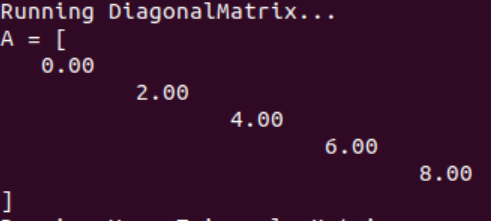
\includegraphics[scale=1]{figures/diagonalmatrix print.png}
        \caption{5-by-5 Diagonal Matrix}
\end{figure}

\subsection{Verification of the Correctness}

\begin{figure}[!ht]
        \centering 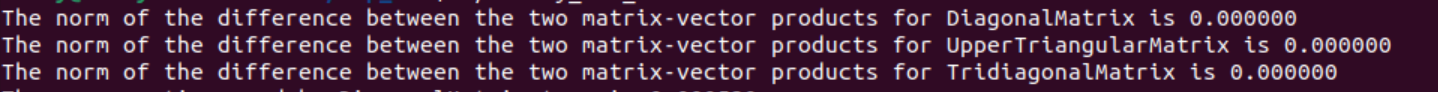
\includegraphics[scale=0.8]{figures/verification.png}
        \caption{Verification}
\end{figure}

The output 0 is the norm of the difference between output vector from multiply\_Matrix\_Vector and output vector from multiply\_DiagonalMatrix\_Vector.

\subsection{Discussion of Implementing Function}

\begin{lstlisting}[]
void multiply_DiagonalMatrix_Vector(Vector* out, DiagonalMatrix* A, Vector* x){  
    for (int i = 0; i < A->n; ++i){    
         out->ptr[i] = 0.0;    
         double A_i = A->ptr[i];    
         double x_i = x->ptr[i];    
         out->ptr[i] += A_i * x_i;  
         }
    }
\end{lstlisting}

Suppose we have a given vector $x$ with length n, and a n-by-n matrix $A$. The output vector is $out$ with length n. $A_{ii}$ is the diagonal entry of row i.
\[
    out_{i} = A_{ii} \times x_{i} \textbf{ for i = 1...n}
\]

\subsection{Comparison of the Runtime}
\begin{figure}[!ht]
        \centering 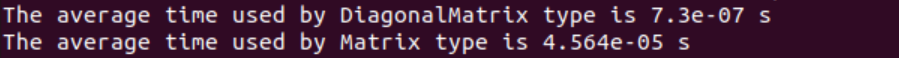
\includegraphics[scale=1]{figures/diagonal runtime.png}
        \caption{Runtime Comparison}
\end{figure}

We can observe that the running time of function with DiagonalMatrix type is a lot faster than the function with Matrix type. The one with Matrix type compute approximately 100$\times$100 times if n = 100, but the one with DiagonalMatrix type compute approximately 100 times, which is faster by roughly factor of 100. 


\section{Upper Triangular Matrix}
\subsection{Output of print}

\begin{figure}[!ht]
        \centering 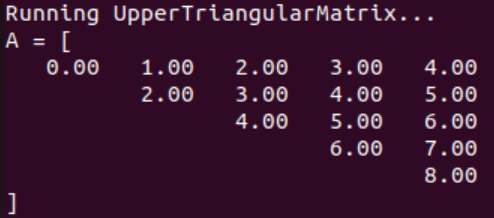
\includegraphics[scale=1]{figures/uppertriangular matrix print.png}
        \caption{5-by-5 Upper Triangular Matrix}
\end{figure}

\subsection{Verification of the Correctness}

\begin{figure}[!ht]
        \centering 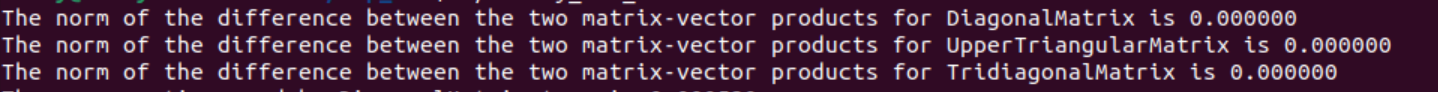
\includegraphics[scale=0.8]{figures/verification.png}
        \caption{Verification}
\end{figure}

The output 0 is the norm of the difference between output vector from multiply\_Matrix\_Vector and output vector from multiply\_UpperTriangularMatrix\_Vector.

\subsection{Discussion of Implementing Function}

\begin{lstlisting}[]
void multiply_UpperTriangularMatrix_Vector(Vector* out, UpperTriangularMatrix* A, 
Vector* x){  
     for (int i = 0; i < A->n; ++i){    
           out->ptr[i] = 0.0;    
           for (int j = i; j < A->n; ++j){      
               double A_ij = A->ptr[i][j];      
               double x_j = x->ptr[j];      
               out->ptr[i] += A_ij * x_j;    
            }  
        }
    }
\end{lstlisting}

Suppose we have a given vector $x$ with length n, and a n-by-n matrix $A$. The output vector is $out$ with length n. 
\[
    out_{i} = \sum_{j=i}^n A_{ij} \times x_{i} \textbf{ for i = 1,...,n}
\]

\subsection{Comparison of the Runtime}
\begin{figure}[!ht]
        \centering 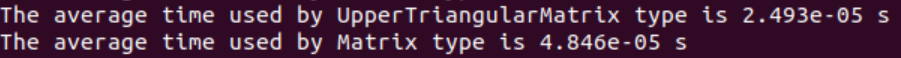
\includegraphics[scale=1]{figures/uppertri runtime.png}
        \caption{Runtime Comparison}
\end{figure}

We can observe that the running time of function with UpperTriangularMatrix type is faster than the function with Matrix type. The one with Matrix type compute approximately 100$\times$100 times if n = 100, but the one with DiagonalMatrix type compute approximately (100$\times$101)/2 times, which is faster by roughly factor of 2. 


\section{Tridiagonal Matrix}
\subsection{Output of print}

\begin{figure}[!ht]
        \centering 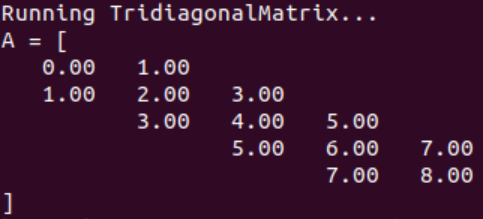
\includegraphics[scale=1]{figures/tridiagonal matrix print.png}
        \caption{5-by-5 Tridiagonal Matrix}
\end{figure}


\subsection{Verification of the Correctness}

\begin{figure}[!ht]
        \centering 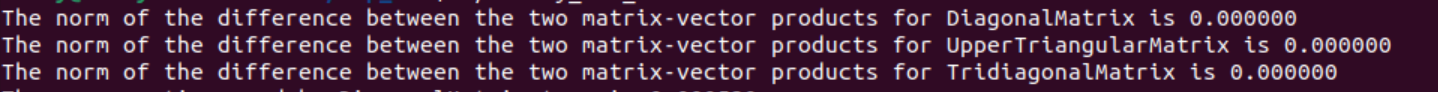
\includegraphics[scale=0.8]{figures/verification.png}
        \caption{Verification}
\end{figure}

The output 0 is the norm of the difference between output vector from multiply\_Matrix\_Vector and output vector from multiply\_TridiagonalMatrix\_Vector.


\subsection{Discussion of Implementing Function}

\begin{lstlisting}[]
void multiply_TridiagonalMatrix_Vector(Vector* out, TridiagonalMatrix* A, Vector* x){ 
    for (int i = 0; i < A->n; ++i){      
        out->ptr[i] = 0.0;      
        if (i==0){          
           out -> ptr[i] = A->ptr_mid[i]*x->ptr[i] + A->ptr_upper[0]*x->ptr[1];      
           }      
        else if (i>0 && i < (A->n)-1){
           out ->ptr[i] = A->ptr_mid[i]*x->ptr[i] + A->ptr_lower[i-1]*x->ptr[i-1]
           + A->ptr_upper[i]*x->ptr[i+1];      
           }       
        else if (i == (A->n)-1){          
           out -> ptr[i] = A->ptr_mid[i]*x->ptr[i] + A->ptr_lower[i-1]*x->ptr[i-1];      
           }    
    }
    }
\end{lstlisting}

Suppose we have a given vector $x$ with length n, and a n-by-n matrix $A$. The output vector is $out$ with length n.
\[
    out_{i} = A_{i1} \times x_{1} + A_{i2} \times x_{2} \textbf{ for i = 1}
\]
\[
    out_{i} = A_{ii} \times x_{i} + A_{i,i-1} \times x_{i-1} + A_{i,i+1} \times x_{i+1} \textbf{ for i = 2,...,n-1}
\]
\[
     out_{i} = A_{i,n} \times x_{n} + A_{i,n-1} \times x_{n-1} \textbf{ for i = n}
\]


\subsection{Comparison of the Runtime}
\begin{figure}[!ht]
        \centering 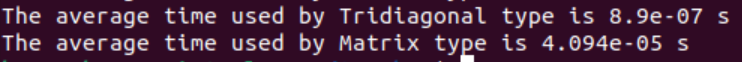
\includegraphics[scale=1]{figures/tridiagonal runtime.png}
        \caption{Runtime Comparison}
\end{figure}

We can observe that the running time of function with TridiagonalMatrix type is a lot faster than the function with Matrix type. The one with Matrix type compute approximately 100$\times$100 times if n = 100, but the one with TridiagonalMatrix type compute approximately 100$\times$3 times, which is faster by roughly factor of 100. 

\end{document}

